\chapter{Psalm 38}

\begin{figure}
  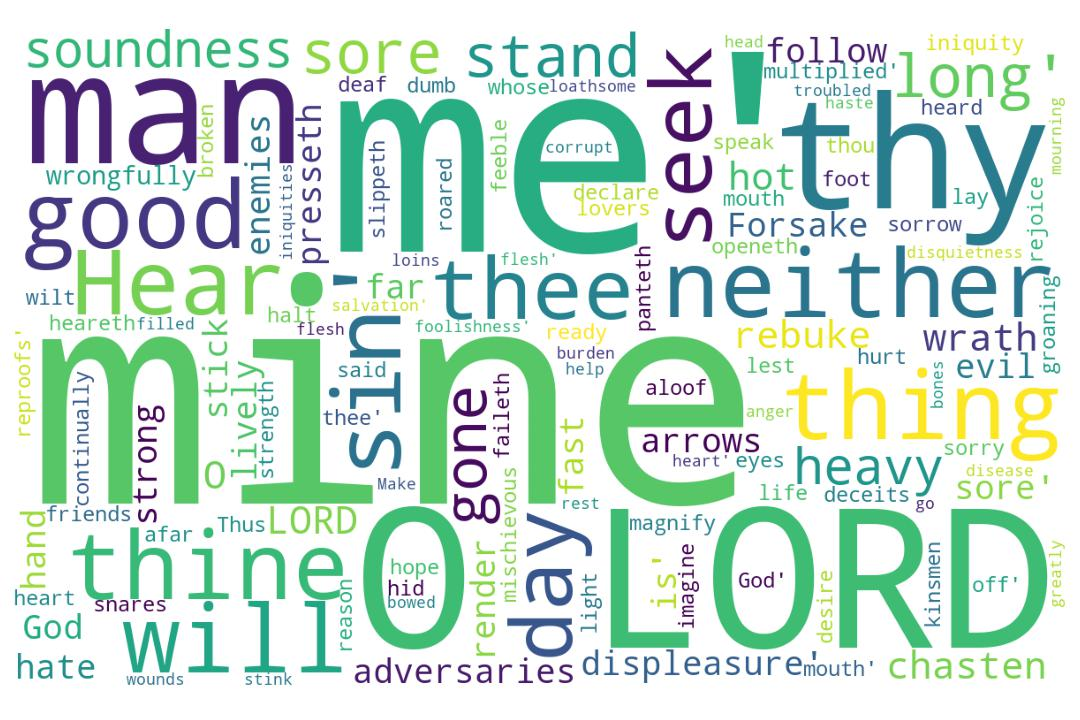
\includegraphics[width=\linewidth]{19OT-Psalms/Psalm38-WordCloud.jpg}
  \caption{Psalm 38 Word Cloud}
  \label{fig:Psalm 38 word Cloud}
\end{figure}

\marginpar{\scriptsize \centering \fcolorbox{bone}{lime}{\textbf{OUT OF SORTS WITH GOD}}\\ (Psalm 38:1-37) \begin{compactenum}[I.][8]
    \item The \textbf{Displeasure} of God \index[scripture]{Psalms!Psa 038:01} (Psa 38:1)
    \item \textbf{Disease} in the Soul \index[scripture]{Psalms!Psa 038:07} (Psa 38:7)
    \item \textbf{Disquietness} in the Soul \index[scripture]{Psalms!Psa 038:08} (Psa 38:8)
    \item A \textbf{Desire} to be Restored \index[scripture]{Psalms!Psa 038:09} (Psa 38:9)
    \item The \textbf{Distance} from Fellowship \index[scripture]{Psalms!Psa 038:11} (Psa 38:11)
    \item The \textbf{Danger \& Deceit} that is present \index[scripture]{Psalms!Psa 038:12} (Psa 38:12)
    \item The \textbf{Declaration} that needs to be Made by Every Man \index[scripture]{Psalms!Psa 038:18} (Psa 38:18)
\end{compactenum}}

\marginpar{\scriptsize \centering \fcolorbox{bone}{yellow}{\textbf{IN THE PLACE OF NEED}}\\ (Psalm 38:1-37) \begin{compactenum}[I.][8]
    \item  \textbf{Daily Chastening}  \index[scripture]{Psalms!Psa 038:01} (Psa 38:1)
    \item \textbf{Distressed Conditions}  \index[scripture]{Psalms!Psa 038:02-03} (Psa 38:2-3)
    \item  \textbf{Dreadful Curruption}  \index[scripture]{Psalms!Psa 038:05} (Psa 38:5)
    \item  \textbf{Deceit \& Cruelty}  \index[scripture]{Psalms!Psa 038:12} (Psa 38:12)
    \item A \textbf{Dire Confession}  \index[scripture]{Psalms!Psa 038:18} (Psa 38:18)
    \item A \textbf{Desperate Call}  \index[scripture]{Psalms!Psa 038:21-22} (Psa 38:21-22)
    %\item Deaf \& Dumb
\end{compactenum}}



\footnote{\textcolor[cmyk]{0.99998,1,0,0}{\hyperlink{TOC}{Return to end of Table of Contents.}}}\footnote{\href{https://audiobible.com/bible/}{\textcolor[cmyk]{0.99998,1,0,0}{Psalms Audio}}}\textcolor[cmyk]{0.99998,1,0,0}{A Psalm of David, to bring to remembrance.}\\
\\
\textcolor[cmyk]{0.99998,1,0,0}{O LORD, rebuke me not in thy \fcolorbox{bone}{lime}{wrath}: neither chasten me in thy hot displeasure.}\footnote{\textbf{Deuteronomy 8:5} - Thou shalt also consider in thine heart, that, as a man chasteneth his son, so the LORD thy God chasteneth thee.}\footnote{\textbf{Job 5:17} - Behold, happy is the man whom God correcteth: therefore despise not thou the chastening of the Almighty:}\footnote{\textbf{1 Corinthians 11:32} - But when we are judged, we are chastened of the Lord, that we should not be condemned with the world.}\footnote{\textbf{Hebrews 12:5-11} - And ye have forgotten the exhortation which speaketh unto you as unto children, My son, despise not thou the chastening of the Lord, nor faint when thou art rebuked of him: [6] For whom the Lord loveth he chasteneth, and scourgeth every son whom he receiveth. [7] If ye endure chastening, God dealeth with you as with sons; for what son is he whom the father chasteneth not? [8] But if ye be without chastisement, whereof all are partakers, then are ye bastards, and not sons. [9] Furthermore we have had fathers of our flesh which corrected us, and we gave them reverence: shall we not much rather be in subjection unto the Father of spirits, and live? [10] For they verily for a few days chastened us after their own pleasure; but he for our profit, that we might be partakers of his holiness. [11] Now no chastening for the present seemeth to be joyous, but grievous: nevertheless afterward it yieldeth the peaceable fruit of righteousness unto them which are exercised thereby.}\footnote{\textbf{Revelation 3:19} - As many as I love, I rebuke and chasten: be zealous therefore, and repent.} %\footnote{The Psalm is called ``A Psalm of David to bring to remembrance.'' Bullinger says that it was used on the Day of Atonement. It is interesting to note that the last four Psalms in the first collection (1--41) have this penitential character about them. There are Messianic references in Psalm 40:7--8, and in Psalm 41:9, but throughout are the troubles of someone who has iniquity and sin in their life that God must deal with (39:1, 40:12, and 41:4). This shows again how carefully the Psalms must be “rightly divided,” and it shows again the extreme carelessness and irreverence of the Alexandrian Cult in dealing with them. Sometimes they cannot even find the spiritual or devotional application (see Psalm 37:4 and 34:11). \cite{Ruckman1992Psalms}}
[2] \textcolor[cmyk]{0.99998,1,0,0}{For thine arrows stick fast in me, and thy hand presseth me sore.}
[3] \textcolor[cmyk]{0.99998,1,0,0}{\emph{There} \emph{is} no soundness in my flesh because of thine anger; neither \emph{is} \emph{there} \emph{any} rest in my bones because of my sin.}\footnote{\textbf{Isaiah 1:6} -From the sole of the foot even unto the head there is no soundness in it; but wounds, and bruises, and putrifying sores: they have not been closed, neither bound up, neither mollified with ointment.} %\footnote{Here we have pictured the agonies of a soul in deep distress. It is David this time, speaking for himself, for the “iniquities” of verse 4 and the “foolishness” of verse 5 are not properties of the Lord Jesus Christ. Verse one reminds us of Hebrews 12:8--12 and should urge the saint to pray for relief from rebuke and chastening, even if they are due and are on the way. He is told to “faint not” and “despise not.” The danger is that the chastening will come in wrath and displeasure instead of love and pity. This chastening (vs. 3) is for sin, and it involves sickness (verses 5, 7), a very grievous sickness like VD or AIDS (see verses 10--11). It may have been something like leprosy, but David calls it a ``loathsome disease.'' Notice the reference in 2 Chronicles 21:15. No weightlifter (Paul Anderson or The Hulk) can bench press sins and iniquities; they are too heavy for anyone to carry except the One who ``taketh away the sin of the world'' (John 1:29) (vs. 4). David’s sickness is brutal for it affected his flesh and bones (vs. 3), his head (vs. 4), his loins (vs. 7), his heart (vs. 8), his eyes (vs. 11), his ears and his mouth (vs. 13), and it brought stinking wounds (vs. 5). Spiritually, you are looking at the condition of a backslidden saint who has been ``snared'' (see 2 Tim. 2:26). He is bowed down; he has no rest; he stinks; he is troubled and diseased; his eyes are dim, and he is deaf and dumb when it comes to hearing God’s instructions or witnessing. The only reason an unsaved man does not feel the burden of sin he is carrying is because he is “dead” (Eph. 2:1--3). \cite{Ruckman1992Psalms}}
[4] \textcolor[cmyk]{0.99998,1,0,0}{For mine iniquities are gone over mine head: as an heavy burden they are too heavy for me.}\footnote{\textbf{Psalm 55:22} - Cast thy burden upon the LORD, and he shall sustain thee: he shall never suffer the righteous to be moved.}\footnote{\textbf{Matthew 11:28-30} - Come unto me, all ye that labour and are heavy laden, and I will give you rest. [29] Take my yoke upon you, and learn of me; for I am meek and lowly in heart: and ye shall find rest unto your souls. [30] For my yoke is easy, and my burden is light.} %\footnote{Verse 4 is the heaviest burden that a man can bear; there is none heavier, and that is why the Lord Jesus said what He said in Matthew 11:28--30. Consider the plight of the lost man—any lost man in any station of life, anywhere: he has to sustain morality without a check on his passions; he has to feel secure about the future without a promise; he has to be happy while feeling guilty; he has to resist the Holy Spirit without a cause, and he has to hope for Heaven while preparing for Hell. Try totin’ that load! I did for twenty-seven years, and when I dumped it by the “wicket gate” (Bunyan) I got rid of a load that would break Hulk Hogan’s back. \cite{Ruckman1992Psalms}} 
[5] \textcolor[cmyk]{0.99998,1,0,0}{My wounds stink \emph{and} are corrupt because of my foolishness.}
[6] \textcolor[cmyk]{0.99998,1,0,0}{\fcolorbox{bone}{bone}{I} am troubled; \fcolorbox{bone}{bone}{I} am bowed down greatly; \fcolorbox{bone}{bone}{I} go mourning all the day long.}
[7] \textcolor[cmyk]{0.99998,1,0,0}{For my loins are filled with a loathsome \fcolorbox{bone}{lime}{\emph{disease}}: and \emph{there} \emph{is} no soundness in my flesh.}\footnote{\textbf{Job 7:5} - My flesh is clothed with worms and clods of dust; my skin is broken, and become loathsome}\footnote{\textbf{Job 7:5} - My flesh is clothed with worms and clods of dust; my skin is broken, and become loathsome.} %\footnote{Kroll prefers to pretend the “loathsome disease” is not in the text. Curtis Hutson, A. V. Henderson, and BBC pretend it isn’t there either (NKJV). The ASV, NASV, NIV, RSV, NRSV, TEV, TLB, NAB, NJB, NWT, RV, etc., all follow suit. (Shortly they will pretend another reading is not in the Psalms. We never have to guess about which verses will be mutilated for we know the character and “godliness” of all of these Fundamental scholars who lost their faith in THE BOOK shortly after being saved.)  \cite{Ruckman1992Psalms}} 
[8] \textcolor[cmyk]{0.99998,1,0,0}{\fcolorbox{bone}{bone}{I} am feeble and sore broken: \fcolorbox{bone}{bone}{I} have roared by reason of the \fcolorbox{bone}{lime}{disquietness} of my heart.}
[9] \textcolor[cmyk]{0.99998,1,0,0}{Lord, all my \fcolorbox{bone}{lime}{desire} \emph{is} before thee; and my groaning is not hid from thee.}
[10] \textcolor[cmyk]{0.99998,1,0,0}{My heart panteth, my strength faileth me: as for the light of mine eyes, it also is gone from me.}\footnote{\textbf{Psalm 13:3} - Consider and hear me, O LORD my God: lighten mine eyes, lest I sleep the sleep of death;}\footnote{\textbf{Psalm 42:1} - As the hart panteth after the water brooks, so panteth my soul after thee, O God.}
[11] \textcolor[cmyk]{0.99998,1,0,0}{My lovers and my friends stand \fcolorbox{bone}{lime}{aloof} from my sore; and my kinsmen stand afar off.}\footnote{\textbf{Psalm 77:2} - In the day of my trouble I sought the Lord: my sore ran in the night, and ceased not: my soul refused to be comforted.}
[12] \textcolor[cmyk]{0.99998,1,0,0}{They also that seek after my life lay snares \emph{for} \emph{me}: and they that seek my hurt speak \fcolorbox{bone}{lime}{mischievous things}, and imagine deceits all the day long.}\footnote{\textbf{Micah 7:3} - That they may do evil with both hands earnestly, the prince asketh, and the judge asketh for a reward; and the great man, he uttereth his mischievous desire: so they wrap it up.}
[13] \textcolor[cmyk]{0.99998,1,0,0}{But \fcolorbox{bone}{bone}{I}, as a deaf \emph{man}, heard not; and \emph{\fcolorbox{bone}{bone}{I}} \emph{was} as a dumb man \emph{that} openeth not his mouth.}
[14] \textcolor[cmyk]{0.99998,1,0,0}{Thus \fcolorbox{bone}{bone}{I} was as a man that heareth not, and in whose mouth \emph{are} no reproofs.} %\footnote{We have already commented on the main things. The important thing to note—which Kroll, Dummelow, Yates, Motyer, et al., all purposely ignore—is the fact that many a saint has to go through what David is going through here. It is not just “David feels that,” or “The Psalmist here expresses....” No, that is no comment at all. The truth is, many a saint has lingered two years in a hospital before he died; many a saint has died alone in a county “rest home,” where no familiar friend showed up more than once every six to ten months; many a saint has had bedsores that stuck to the sheet; many a saint was so weak for months that he could not lift up a fork; and many a saint was abandoned by his family and his wife (or her husband) and then was the subject of common gossip all over the community (vs. 12). The commentators—knowing nothing about these things (see The Last Grenade, Ruckman [Pensacola: Bible Baptist Bookstore, 1990], pp. 325–334) trip merrily on, pretending that everything is either “Messianic” or historical. Life is real. The Bible is real. David is not just describing his own condition. The Holy Spirit is describing the mess you may find yourself in some day. If you do get in this mess what you will need is this Psalm; not some lost scraps of paper that might (or might not) be mistaken (or identified) as “original autographs.” The scholars are naive: naive, and stupid as well. Someone may want you to die to get your money (vs. 12), and they may have Medicare, or a doctor, or the HEW, or “Prudential” to help “set things up.” There is nothing limited about David’s problems. God has shut David’s mouth so that he cannot witness (vss. 13–14). Paul was tempted to do this on occasion; subsequently, he covets the prayers of the saints that he might keep on speaking up boldly when his circumstances would dictate silence (Eph. 6:19). David cannot rebuke his adversaries and betrayers because God has slapped him down. He cannot accept their suggestions or criticisms (vs. 13) because they solve nothing. He is in Job’s condition (Job 30:9–17), where God is the only One he can appeal to (Job 10:1–8). You will find yourself in THAT condition if God ever uses you one fourth as much as He used David. Note one historical incident for verse 14: David does not rebuke Shimei for cursing him (2 Sam. 16:11–13). \cite{Ruckman1992Psalms}}
[15] \textcolor[cmyk]{0.99998,1,0,0}{For in thee, O LORD, do \fcolorbox{bone}{bone}{I} hope: thou wilt hear, O Lord my God.}\footnote{\textbf{Psalm 17:6} - I have called upon thee, for thou wilt hear me, O God: incline thine ear unto me, and hear my speech.} %\footnote{Verse 15 is the sentiment of Psalm 39:7: “What wait I for? my hope is in thee.” No hope in his lovers (vs. 11). No hope in his friends (vs. 11). No hope in his relatives and family (vs. 11). No hope in his enemies (vs. 12). No hope in his physical condition (vss. 7–10), and no hope in the POPE! “Rome enslaves; Jesus saves.” Aside from God hearing him and helping him, he is hopeless. David is sorry for his sins; this is the true penitent who is not just sorry for having been caught (see Judas, Pharaoh, and Balaam), but is sorry for what he IS (see Job 42:6) as well as what he has done (Luke 15:18, 20). All is in order for a sinning saint in the twentieth century in spite of the “Dry Cleaners.” These ultra-dispensationalists teach that no Christian should confess sins or ask for forgiveness for them since “Calvary covers it all.” A real “Hyper,” like E. C. Moore or A. Watkins, believes that if you get baptized in water you are an “enemy of the cross of Christ” and have made the “preaching of the cross” of no effect: ditto when you confess your sins. Not all the clowns are in the circus. If God’s enemies rejoice when you get in trouble, then your best bet after confessing your sins, judging them, and forsaking them, is to appeal to God’s interest in you as His servant, doing His work for His glory (vss. 15–17). It is useless to appeal to your own righteousness. \cite{Ruckman1992Psalms}}
[16] \textcolor[cmyk]{0.99998,1,0,0}{For \fcolorbox{bone}{bone}{I} said, \emph{Hear} \emph{me}, lest \emph{otherwise} they should rejoice over me: when my foot slippeth, they magnify \emph{themselves} against me.}\footnote{\textbf{Psalm 35:26} - Let them be ashamed and brought to confusion together that rejoice at mine hurt: let them be clothed with shame and dishonour that magnify themselves against me.}
[17] \textcolor[cmyk]{0.99998,1,0,0}{For \fcolorbox{bone}{bone}{I} \emph{am} ready to halt, and my sorrow \emph{is} continually before me.}
[18] \textcolor[cmyk]{0.99998,1,0,0}{For \fcolorbox{bone}{bone}{I} will \fcolorbox{bone}{lime}{declare} mine iniquity; \fcolorbox{bone}{bone}{I} will be sorry for my sin.}
[19] \textcolor[cmyk]{0.99998,1,0,0}{But mine enemies \emph{are} lively, \emph{and} they are strong: and they that hate me wrongfully are multiplied.}
[20] \textcolor[cmyk]{0.99998,1,0,0}{They also that render evil for good are mine adversaries; because I follow \emph{the} \emph{thing} \emph{that} good \emph{is}.}\footnote{\textbf{Proverb 17:13} - Whoso rewardeth evil for good, evil shall not depart from his house.} %\footnote{Notice that a saint can be sinning when he is on the right way trying to do right (vs. 20). Notice also that his sins are between him and God, and that he can be hated for right actions even while he is out of fellowship with God (vss. 19–20). These two tremendous New Testament doctrinal and practical truths escape the eyes of Kroll, Motyer, Dummelow, Ellicott, Jamieson, Fausset, Brown, Briggs, Davidson, and Keil, exactly as they escaped the notice of Yates, Baethgen, Sumner, Freerksen, Wemp, Kutilek, Clarke, Lange, Williams, Hitzig, and Hupfeld. \cite{Ruckman1992Psalms}} 
[21] \textcolor[cmyk]{0.99998,1,0,0}{Forsake me not, O LORD: O my God, be not far from me.}\footnote{\textbf{Matthew 27:46} - And about the ninth hour Jesus cried with a loud voice, saying, Eli, Eli, lama sabachthani?  that is to say, My God, my God, why hast thou forsaken me?}\footnote{\textbf{Mark 15:34} - And at the ninth hour Jesus cried with a loud voice, saying, Eloi, Eloi, lama sabachthani? which is, being interpreted, My God, my God, why hast thou forsaken me?}
[22] \textcolor[cmyk]{0.99998,1,0,0}{Make haste to help me, O Lord my salvation.}\footnote{\textbf{Psalm 40:13} - Be pleased, O LORD, to deliver me: O LORD, make haste to help me.}\footnote{\textbf{Psalm 70} - Make haste, O God, to deliver me; make haste to help me, O LORD. [2] Let them be ashamed and confounded that seek after my soul: let them be turned backward, and put to confusion, that desire my hurt. [3] Let them be turned back for a reward of their shame that say, Aha, aha. [4] Let all those that seek thee rejoice and be glad in thee: and let such as love thy salvation say continually, Let God be magnified. [5] But I am poor and needy: make haste unto me, O God: thou art my help and my deliverer; O LORD, make no tarrying.}\footnote{\textbf{Psalm 71:12} - O God, be not far from me: O my God, make haste for my help.}\footnote{\textbf{Psalm 141:1} - LORD, I cry unto thee: make haste unto me; give ear unto my voice, when I cry unto thee.}






